\documentclass[pdftex,12pt,letter]{article}
\usepackage[binary-units=true]{siunitx}
\usepackage[margin=0.75in]{geometry}
\usepackage{verbatim}
\usepackage{graphicx}
\usepackage{cite}
\usepackage{color}
\usepackage[pdftex,pdfpagelabels,bookmarks,hyperindex,hyperfigures]{hyperref}
\usepackage{xspace}
\usepackage{amssymb}
\usepackage{authblk}

\bibliographystyle{unsrt}

\newcommand{\fixme}[1]{\textbf{FIXME: #1}}    
\newcommand{\pd}{protoDUNE\xspace}
\newcommand{\dtpc}{\textit{dunetpc}\xspace}

\title{Report from ProtoDUNE Single-Phase Data Challenge 1}
\date{\today}

\author{S. Fuess, A. Mazzacane,  I. Mandrichenko, R.Pordes,  A. Norman, J.Paley \\
M.Potekhin, G. Savage, H. Schellman, D. Stefan, R.Sulej, S. Timm}


\begin{document}
\maketitle
\begin{abstract}
\noindent We report on the first ProtoDUNE Single Phase Data Challenge that took place in November 2017
\end{abstract}


\begin{itemize}
\item Version 0.1: Initial report draft - missing sections on components still to complete.
\clearpage
\end{itemize}

\tableofcontents
\pagebreak



\section{Introduction and Overview}

The first Data Challenge  (DC1) took place the week of November 6th. The overall goal was to test the functionality and interfaces of main components of the offline infrastructure solutions.  Interfaces to the data sources in EHN1 (DAQ, Online and Beam Instrumentation) were emulated or provided via test components. 
\subsection  {Scope}

The components of the overall offline system that were included in the Data Challenge were:
\begin{itemize}


\item 25 Terabytes of already reconstructed simulation data files from Monte Carlo Challenge 9 were available on EOS at the CERN Tier-0.
In total 28 TB  were copied (some files were copied more than once) using F-FTS-Light running on an OpenStack VM to an EOS data buffer.
From there they were copied using F-FTS to the Data Quality Monitoring dropbox/input buffer, to tape at CERN (on Castor) and Fermilab
(on Enstore) and to disk at Fermilab (dCache). 

\item   The \textit{protoDUNE prompt processing system} (p3s) operated throughout DC1. Its primary goal was to support
the Data Quality Monitoring (DQM)  functionality in \pd by running detector characterization algorithms with a short turnaround time.
The system worked by automatically detecting new input files and running 3 applications on each file: the purity monitor,
noise filtering and event display, and the CRT track matching. 

\item A POMS campaign for processing the files arriving at Fermilab was run in three phases: the first with just the infrastructure
of the current \dtpc to read in and write out the data; the second to introducing the art/LArSoft infrastructure and the third with the full current payload for the
upcoming protoDUNE-SP Monte Carlo Challenge 10. 

\item In parallel fake data was loaded into the IFBEAM Beam Instrumentation database and existing LHC Beam Line data was ingested into IFBEAM by transfering data from CERN.

\item An initial attempt to run a user \dtpc job using the  usual project.py interface to running grid jobs at Fermilab was
attempted using the site CERN (Tier-0) and a data file stored in Castor provided to the job locally (i.e.~without transferring
the data back from Fermilab to the CERN EOS). 

\item Information about output displays and web pages, monitoring web pages and information, was collected on the wiki.dunescience.org

\end{itemize}

 Fig.\ref{fig:dependencies} shows the components of the end-to-end system and their dependencies. Fig. \ref{fig:intermediate} shows those components included in the Data Challenge. 


\begin{figure}[tbh]
  \centering
  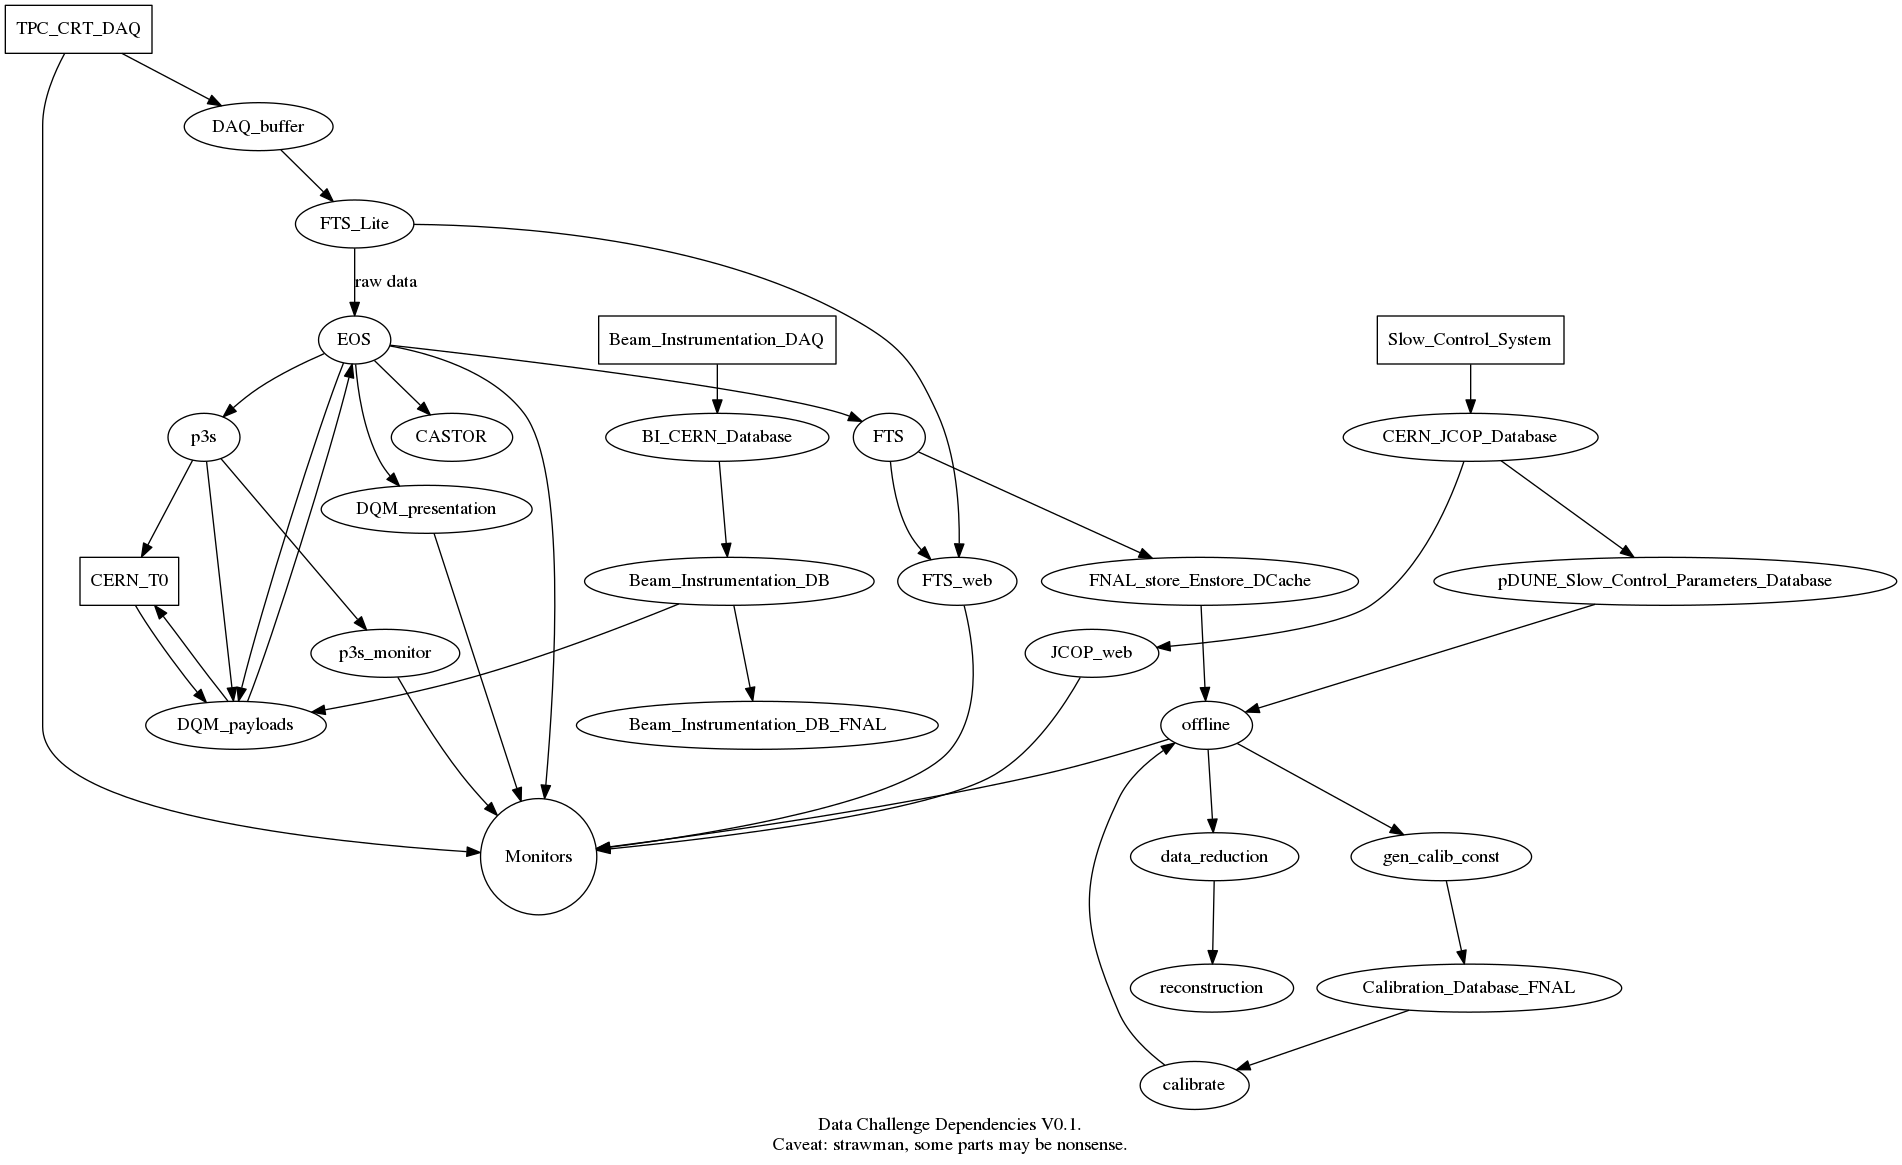
\includegraphics[width=0.75\textwidth]{../figures/dc1_integration.png}
  \caption{Schematic of Dependencies}
  \label{fig:dependencies}
\end{figure}


\begin{figure}[tbh]
  \centering
  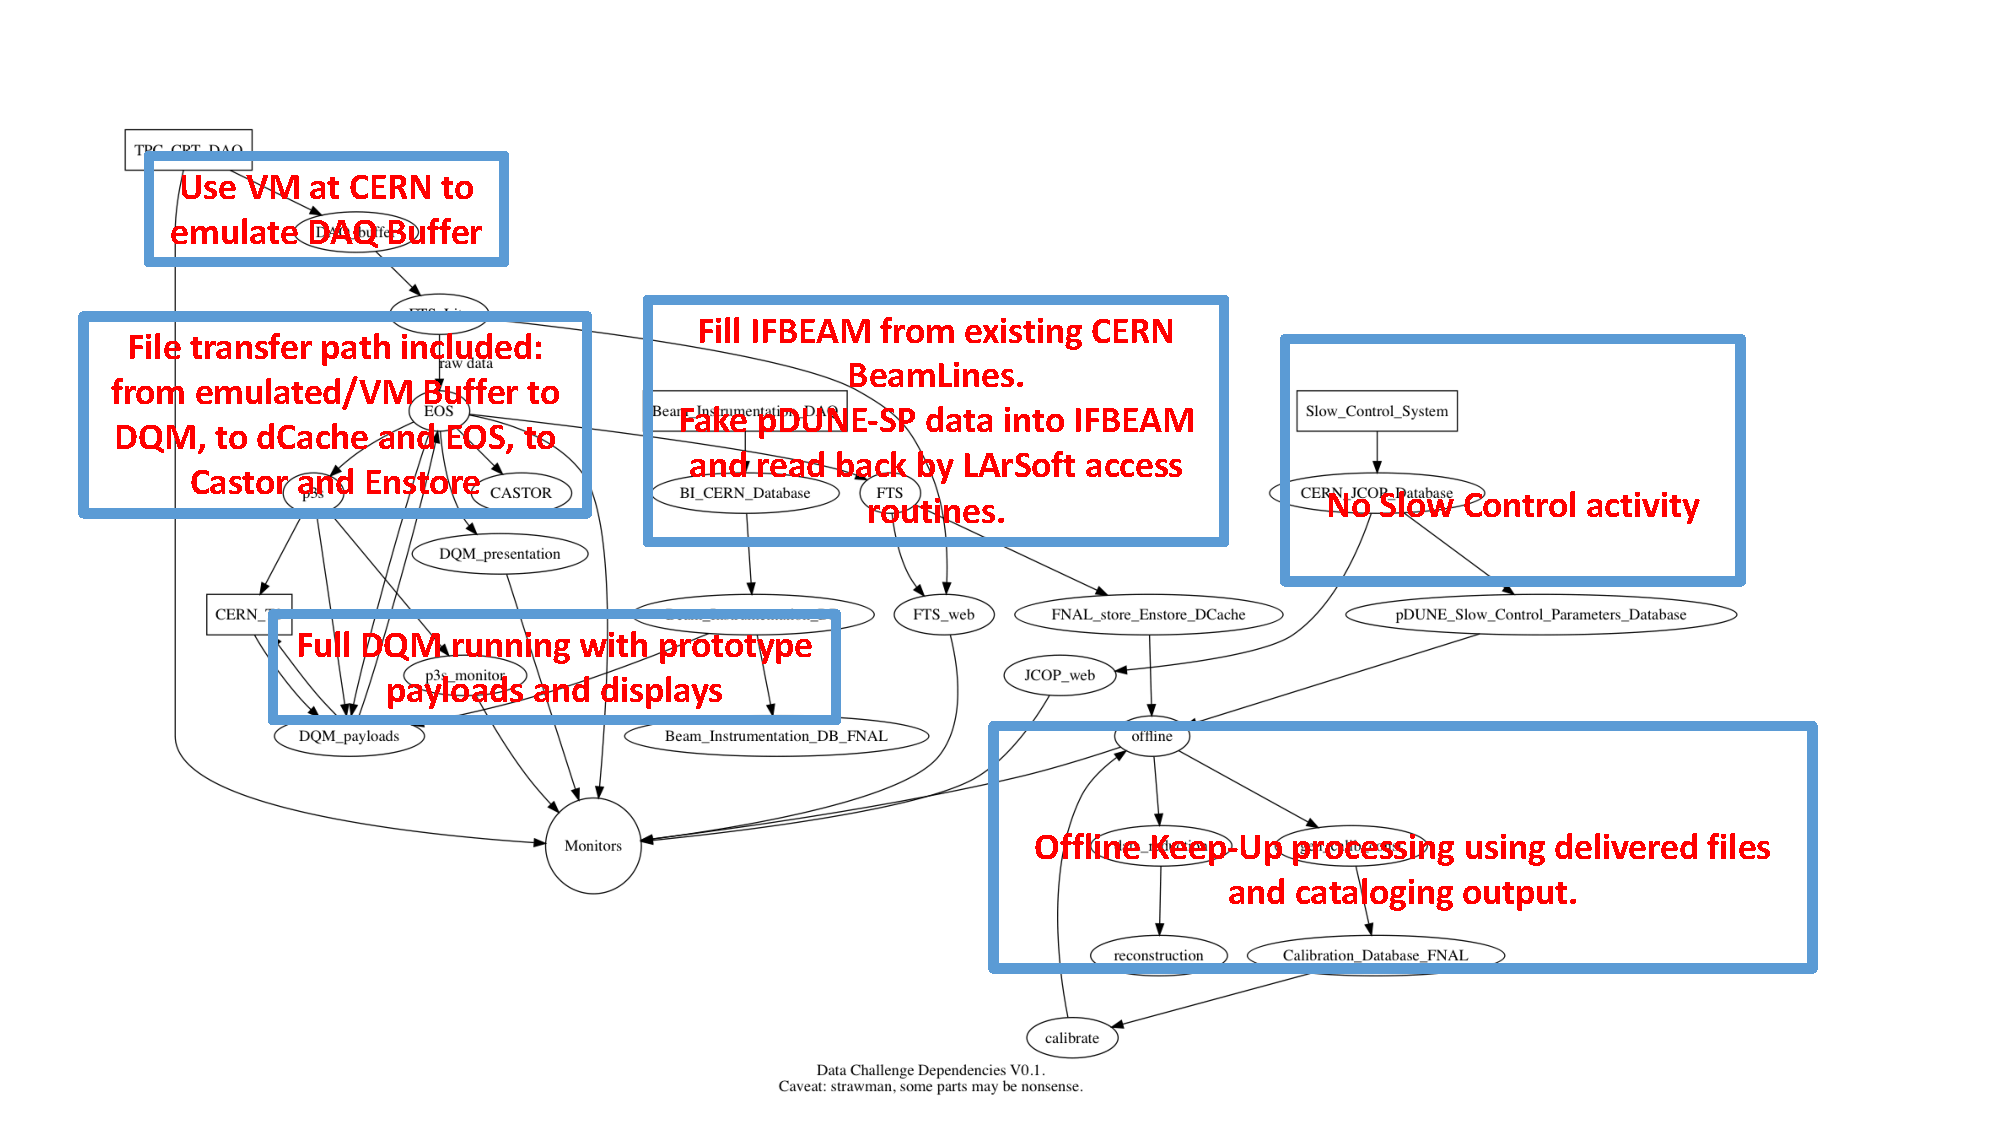
\includegraphics[width=0.75\textwidth]{./ReportImages/intermediate.pdf}
  \caption{What was included in the Data Challenge 1}
  \label{fig:intermediate}
\end{figure}

\subsection {Outside of Scope}

The scope of this data challenge did not include assessing the overall throughput, sustainability, and performance  of the system. However,  the groups running each of the components  analyzed  the latency, throughput and robustness of their software and services. This was a very valuable outcome of the work,   together with debugging and identifying problems and solutions. 




\section {Data Movement}
\subsection {Definitions}
F-FTS refers to the Fermi File Transfer Service, the standard Fermilab utility which is used to transfer files from a DAQ system to permanent storage and declare them to SAM (Sequential Access with Metadata) database.  F-FTS-Light is a similar program but can operate behind a private net or firewall and does not need to be in contact with SAM or anything else at Fermilab.

The event data used was the dataset of MCC9 data set already available on disk at the CERN EOS, which consisted of
23TBytes,  ~3000 files of average size 8GB, with the data being in  "mergeana" (post merging/processing)  format. There were 
40 subdirectories each corresponding to a different beam energy and with or without the simulation of the space charge effect.

\subsection{Initial Copy Script Details}
From the original location of the MCC9 file  an initial copy script (copy\_mcc9\_data.py): took the files to the simulated DAQ buffer in the EOS file cache via 3rd party xrdcp; added a process ID and a timestamp to the filename; and was configured to ensure a maximum rate at which the xrdcp happened at some point doing the test. It also created a rudimentary set of metadata,

The script could also be configured to stagger copies of files for N seconds between each one or be asked for a specific  count of files. As part of the copy new (SAM) metadata was created. This initial copy broke the 40 directories into 4 chunks and copied 10 directories at once into the buffer, for the goal rate of 500MB/s. As a side-product the test ended up twice launching 5 copies of the copy script rather than one, so 50 xrdcp commands were going at once on the first two days of the DC. This all worked fine with nothing breaking down. See Fig.\ref{fig:EOStoEOS} for monitoring information of the copy. 


\begin{figure}[tbh]
  \centering
  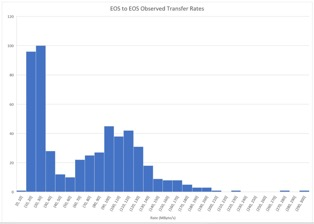
\includegraphics[width=0.5\textwidth]{./ReportImages/EOStoEOS.jpg}
  \caption{EOS to EOS Copy Monitoring}
  \label{fig:EOStoEOS}
\end{figure}

\subsection{F-FTS and F-FTS-Light Operation}
From the emulated DAQ buffer in EOS, F-FTS-Light was used to transfer files into the F-FTS dropbox which was also in EOS.  F-FTS-Light also used 3rd-party xrdcp as its means of file discovery and transport.  It transferred the file, received the checksum that was returned from the xrdcp command, and then added it to the metadata.  Throughout the course of this challenge, F-FTS-Light was configured to transfer 10 files in parallel.   When 10 copy scripts were running upstream, F-FTS-Light was able to keep up to that data flow.  For this test F-FTS-Light ran on an OpenStack VM with 2 cores.  It will eventually run on a server in EHN-1.

For the purposes of this test F-FTS was configured with three destinations:  the input dropbox of the prompt processing P3S, which was also in EOS, Castor tape servers, and dCache/Enstore at CERN.  F-FTS also runs on an OpenStack VM.
For the EOS-to-EOS copy and the EOS-to-Castor copy, 3rd-party xrdcp was used.  For the EOS-to-Fermilab copy we used 3rd party gridftp (globus-url-copy).
FTS was configured to make 10 transfers in parallel to each of the three destinations. Files were declared to the dc1\_input data set in SAM.



\subsection{Results and Observations}
The full set of data files was moved to the 2 archival facilities over the period of about 5 days.  This included gaps of several hours during each day when we did not start any new copies. There were a variety of throughput rates sustained. Changes in configuration of the CERN EOS interface helped with stability of the scripts/services being run. 

On the CERN side an aggregate rate of 200MByte/s was sustained. FTS-Light kept up with the input files, which means it can also handle sending at that rate from the detector. (These rates can be increased by adding more xrdcp processes as needed). Individual file transfer rates show a bimodal distribution due to the fact that some files are stored at Wigner and some at Meyrin.  See \ref{fig:FTSLite}


\begin{figure}[tbh]
  \centering
  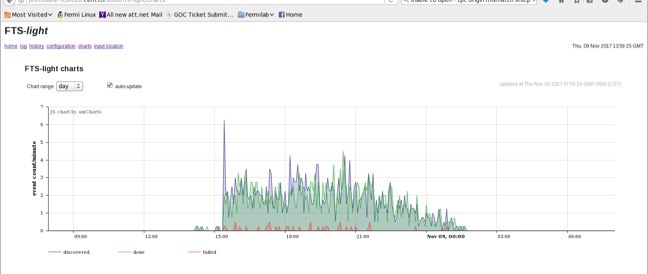
\includegraphics[width=0.5\textwidth]{./ReportImages/FTSLite.jpg}
  \caption{FTS Lite transfer monitoring}
  \label{fig:FTSLite}
\end{figure}


On the CERN Tier-0 the monitoring showed that the EOS traffic generated clearly dominated the EOS accessed during the time of the tests without crashing any EOS servers. (For short periods the monitoring showed that the EOS can even take much higher influx and then recover.)

For the transfers from CERN EOS to Fermilab dCache the best 1/2 hr average we saw to Fermilab about 180MByte/sec. Rates of each stage of the file movement, archiving and declaration to the SAM metadata catalog are shown in  Fig.\ref{fig:FTStoFermilab}

Note that the Eospublicftp gateways in use to copy the data from CERN to Fermilab should be able to source more than that. The parallelism was kept to 10 simultaneous globus-url-copy processes for this test. We have  been advised by CERN experts that this should be able to scale up by a factor of 10.  This should allow the full rate needed for the protoDUNEs to be achieved. In addition, further tests will be done to measure how far the scaling can be done.


\begin{figure}[tbh]
  \centering
  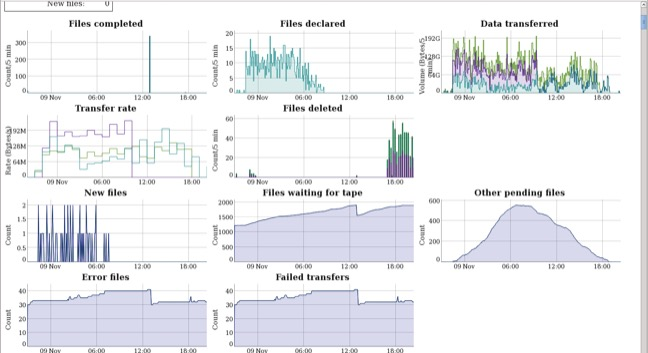
\includegraphics[width=0.5\textwidth]{./ReportImages/FTS.jpg}
  \caption{Monitoring of FTS copies}
  \label{fig:FTStoFermilab}
  
\end{figure}. 



\subsection {Future Work}
We clearly need to test data transfers originating from a disk on the EHN1 network - preferably from the pDUNE-SP and pDUNE-DP event data buffers. 

We need to converge on  the details of the metadata format and who writes it. It is currently agreed that this is provided by the DAQ/Online Group and they will write it. We hope the first test can be used to test this also. 

We need to move the FTS Virtual Machine from a private project OpenStack to the  DUNE OpenStack project. 

For the test the files moved to the DQM were declared to SAM since that is what FTS automatically does. We need to define the configuration of and move the files relevent to the DQM inbox without declaring them to SAM. From that point the DQM is responsible for their management.

We plan to clean this data challenge data set off of tape and SAM when the keep-up processing is completed.


\section {Data Quality Monitoring}
DC1 was an extremely useful exercise which helped to test and demonstrate the Data Quality Monitoring component
of the ProtoDUNE Single Phase offline system. Overall this was a success.

\subsection{Work-Up}

During the work-up to DC1 the week before, the following was validated
\begin{itemize}

\item The p3s infrastructure was pushed to utilize 1000 cores in CERN Tier-0 and kept that level of resource utilization for ~1hr
with realistic payloads
\item It was verified that p3s can accept jobs (means Apache and DB throughput) at ~100Hz rate

\end{itemize}
\noindent Technically this levels of throughput was not required in DC1 but it was considered important to know the system capability.
Characteristics of the HTCondor batch system in CERN Tier-0 were studied from the point of view of the DQM job sumbission and
execution.

In addition, automation for data discovery was created with periodic polling of the p3s ``inbox'' for new data according to a predefined pattern
and registration of these data for processing in the system. The p3s GUI was simplified and cleaned up. The current look of the p3s
dashboard screen is presented in Fig.\ref{fig:p3s_dash}.
\begin{figure}[tbh]
  \centering
  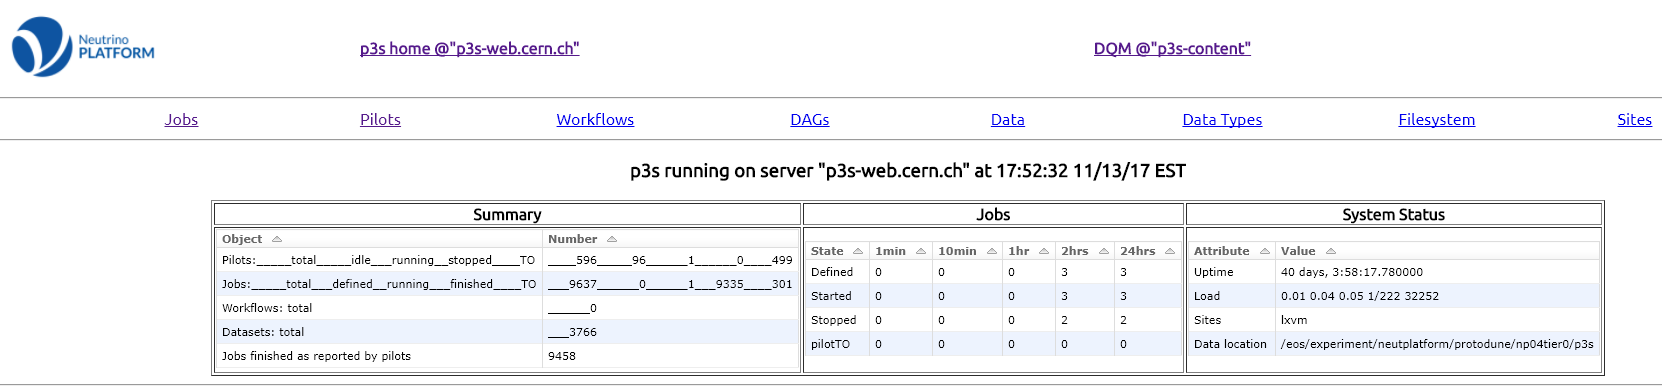
\includegraphics[width=1.0\textwidth]{./ReportImages/p3s_20171113_1.png}
  \caption{The p3s dashboard}
  \label{fig:p3s_dash}
\end{figure}

\subsection{Operation}
The p3s/DQM component of the Data Challenge remained operational throughout the testing period with virtually no human intervention.
It was monitored through its GUI and log files, and a few infrastructure issues that were discovered (see \ref{sec:p3s_issues}) were communicated
to CERN ITD. The DQM processing kept up with the nominal data rate dictated by the rate of data transmission of DC1, with substantial headroom in
terms of the load on the p3s servers and also in terms of computing power available in CERN Tier-0.

\subsection{Payloads}
Three kinds of DQM payloads were used during DC1:
\begin{itemize}

\item A simple Event Display (channel vs time for each TPC section) combined with signal processing
and filtering (provided by David Adams)
\item Purity Monitor (estimation of the electron lifetime based on a group of tracks, provided by Bruce Baller). The software is described in a presentation \href{https://indico.fnal.gov/event/14840/contribution/0/material/slides/0.pdf}{here}.

\item CRT-to-TPC track match (tracking with Cosmic Ray Tagger and correlation with TPC,  provided by Joe Prividi). The software is described in a presentation \href{https://indico.fnal.gov/event/13293/session/6/contribution/112/material/slides/0.pdf}{here}

\end{itemize}
\noindent These payloads performed without apparent failures. An example of the Event Display output
is presented in Fig.\ref{fig:evdisp}, demonstrating the functionality of this application.
\begin{figure}[tbh]
  \centering
  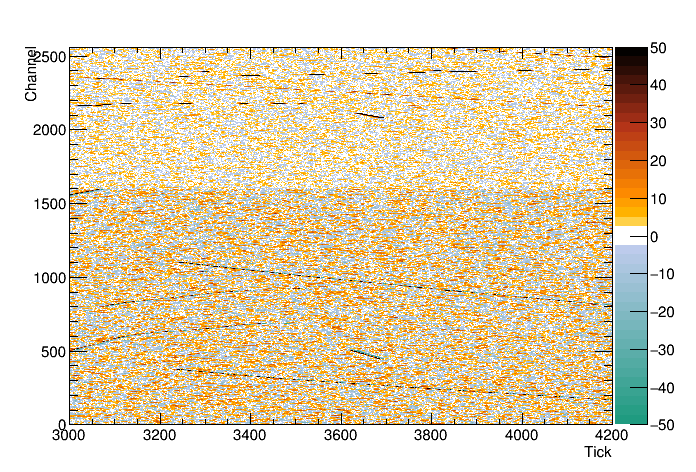
\includegraphics[width=0.6\textwidth]{./ReportImages/adcraw_evt33_ch0-2559.png}
  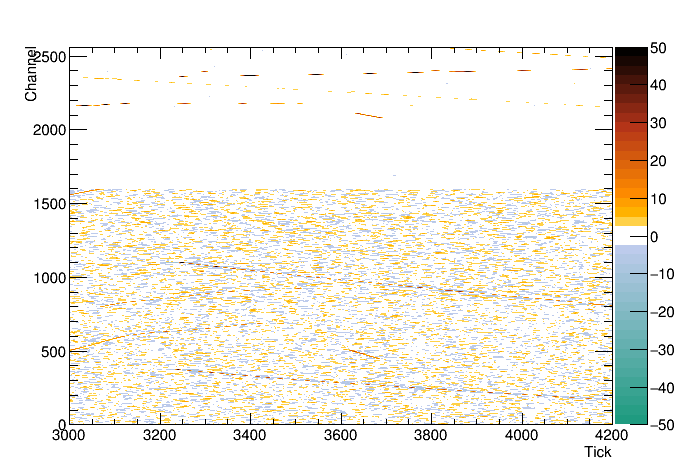
\includegraphics[width=0.6\textwidth]{./ReportImages/adcprep_evt33_ch0-2559.png}

  \caption{Event Display of same event before and after signal processing}
  \label{fig:evdisp}
\end{figure}

\noindent  A an auxiliary "presentation server" p3s-content.cern.ch
was used to serve the event display images and timestamped purity tables.

\subsection{Mode of Data Access}
The mode of data access by the payload jobs running on Worker Nodes (both input and output) was the FUSE mount of EOS.
Depending on the results of future data challenges this may provide enough performance and
stability for the \pd operations. If proven otherwise, migration to XRootD interface (such as \textit{xrdcp})
will be considered.

The specific method by which the input data are placed in the p3s ``inbox'' is outside of the p3s scope and is
under the umbrella of the FTS/Data Handling Team.

The presentation Web service was also accessing the DQM outputs via the FUSE mount which was 
soft linked to a directory included in the Apache server configuration. No problems were detected
with this setup during DC1.



\subsection{Problems encountered}
\label{sec:p3s_issues}
Problems enountered during the Data Challenge are outlined below. While some of them were serious, none
were severe enough to disable p3s or critically slow it down. While the efficiency dropped on one occassion to 70\% due to an AFS problem
this was an isolated incident and was not typical for the test period as a whole. Still, it is prudent to keep an eye
open for similar issues in future data challenges and to develop fixes, workarounds and other types of mitigation
to the fullest extent possible.

\subsubsection{AFS}

In DC1 AFS was not used as either temporary or principal data store for either emulated raw data or DQM data products.
It was used to host two types of software in p3s/DQM:
\begin{itemize}
\item p3s client software i.e.~a collection of Python and shell scripts driving the p3s server, performing service duties etc
\item local builds of DQM software e.g. duneTPC
\end{itemize}

\noindent In each case the software was hosted in the user space i.e.~the partition of AFS reserved for interactive sessions
and which is not typically meant to be accessed by a large number of worker nodes etc. There is a separate class
of AFS storage (``work space'') which has different characteristics and which may behave differently, which would
be an action item for continued testing in DC1 etc.

In DC1 there was a period when there were indications of AFS clients losing connectivity/timing out.
This happened in fraction of cases which variable over time and is not specific to p3s, as it has also reported
by the DRA group in a separate activity. This type of malfunction may result in the "bus error" message and crashes of
pilot jobs used in p3s for workload management. The were occasional report about pats not found which are likely
related to the same root cause. Conculsting with CERN ITD via the ticket system did not produce definitive results.

We must look into optimizing access patterns to the code deployed in AFS.

\subsubsection{EOS}
Problems enountered with EOS were all due to the FUSE system and not to the underlying storage or XRootD.

\begin{itemize}

\item Infrequent filesystem errors when periodically flushing certain directories in EOS. This does not happen often (e.g. approx at 0.1\% level).
Root cause has not been established by CERN ITD. Native EOS interface did work as expected for deletion of directories.

\item Occasional failure to find a path in EOS. The frequency of this occurrence has not been quantified but it was not large.

\item At the time of writing, inability to use EOS to keep HTCondor log files (see below).

\end{itemize}



\subsubsection{HTCondor}
\begin{itemize}

\item Condor vacating pilot jobs i.e. not respecting the required time limit. Filed a ticket. An error was found in the Condor configuration, testing ongoing.

\item Ongoing problems with the FUSE mount when used at scale lead to cropping up of HTCondor problems when for a example a COndor
process needs to keep its log file in EOS via FUSE. This has led to substantial problems to part of the Tier-0 HTCondor infrastructure and
resulted in enforcement of policy which forbids dependency of Condor submission (at the level of stdout, stderr and log) on EOS/FUSE.
This has happened immediately after completion of DC1 and may be an issue going forward. A fix is promised in early 2018. Until then,
the current recommendation is to use AFS for such purposes.

\end{itemize}

 
\subsection{Directions for future work}

\begin{itemize}

\item Request from DRA to support workflows in p3s with LArSoft payloads. The DAG-style workflow mechanism in p3
(including a library of workflow templates) has been implemented a while ago but not tested with realistic payloads and/or at scale.

\item Work with the DRA group to identify, create, test and deploy other crucial payloads as a part of the \pd DQM portfolio.

\item The "basic metadata" issue i.e. how to cross reference DQM outputs and raw data. This can be the sub-event level such as the event
display for a single APA in a particular run/subrun/event. Alternatively, the purity data must refer to a list of events and run number in reference
to actual raw data. This is very different from the "Metadata" in the sense of the word we are typically using e.g. SAM etc.
It is a product of DQM rather than of the data handling system. Need "standard" JSON schemas and tools to facilitate this work for payload developers.

\item Beam Instrumentation payloads have not been tested in DQM. This is upon the BI/DRA groups to implement.

\item Migration of p3s Web and DB services from personal to group/production accounts.

\item Easy to access, efficient documentation for shifters evailable from the p3s pages.

\item Miscellaneous imporovements in the GUI.

\item Archiving of older DB entries to shrink active tables and preserve performance.

\item Interfacing SAM/FTS for archiving of selected DQM outputs.

\item Policies and tools for cleaning out input/output storage areas.

\item Logging of external events (i.e. output of services managing the HTCondor submission, data cleanup etc) in a proper database
in p3s itself as opposed to string of e-mail coming from cron. This work has already started.

\end{itemize}

\subsection{Summary}
The \textit{ \pd prompt processing system} performed well and in a stable manner during DC1. It has proven itself as a solid tool for addressing the Data Quality Monitoring needs
of \pd. A few infrastructure issues have been identified and are being addressed.
Directions for future work have been defined.
 


\section {Keepup Processing}

The Data Challenge 1 Keepup Processing  included end to end testing of the offline processing infrastructure, physics payloads to be used for reconstructed simulation data in the upcoming Monte Carlo challenge, and declaration of output files back into the catalog and archival storage.  
In order to decouple infrastructure issues from  payloads problems, it was agreed to split the Data Challenge into three phases and run the processing more than a week if needed:
\begin {itemize}

\item Phase 1: Simple  ''null" job.\\
 This phase consists of the copy the file in  from the SAM input dataset, sleeps for a well defined amount of time, renames the file and copies it out with appropriate metadata to the offline dropbox.\\
This stage is designed to completely decouple from ANY art or LarSoft dependancies or reconstruction code. 


\item Phase 2: Simple art/Larsoft based "null" jobs.\\
 In this phase the Lar executable is introduced to run using a fcl file. As in the previous stage, the processing consists of the copy in and the copy out after a delay of a well amount of time that mimic the reconstruction time. \\
 This stage is designed to identify any potential problems with the use of the experiment framework and workflows, but NOT be dependent on a specific set of reconstruction algorithms.  


\item Phase 3: Full payload art/Larsoft "mini-reco" jobs.\\
 This phase consists of running  a mini-reco processing using payloads provided by Robert and Dorota. \\
 Respect the real simulated daq  data, the processing of the mcc9 files as input dataset required the stripping of all info, but the simulation and the digitization of the data event.

\end{itemize}

\subsection {Preparation}

During the preparation phase, POMS campaigns and configurations scripts are created and tested.
For each campaign, a keepup processing is setup to run every 4 hours (6 submission/24 hours).
At each submission, all new files  copied in the input SAM dataset at FANL are processed.
The output files are renamed and copied with appropriate metadata to the offline dropbox where an FTS instance is configured to copy them on tape (@FNAL and @CERN).
POMS is also configured to automatically  recover data files that were not processed.
Configurations scripts were created to submit grid jobs on the FermiGrid using jobsub without the additional layer of project.py  that is usually used for DUNE/pDUNE  Monte Carlo production.
This step required some more work but with the advantage of a better control of the entire workflow.

\subsection {Processing}

\begin{itemize}
\item Phase 1: Copy in, then Copy out, with a 2 min sleep between them.\\
The keepup processing ran smoothly after several fine tunings.
A bug related to the input dataset (there was no control that input files were actually copied to FNAL) where found and immediately fixed.
The stable processing started on November 8th, followed by a submission every 4 hours. 
The SAM projects for each submission (keepup and recovery) are  the links shown in the second column of the POMS webpage (Fig.\ref{fig:keepupprocessingphase1}).


\begin{figure}[tbh]
  \centering
  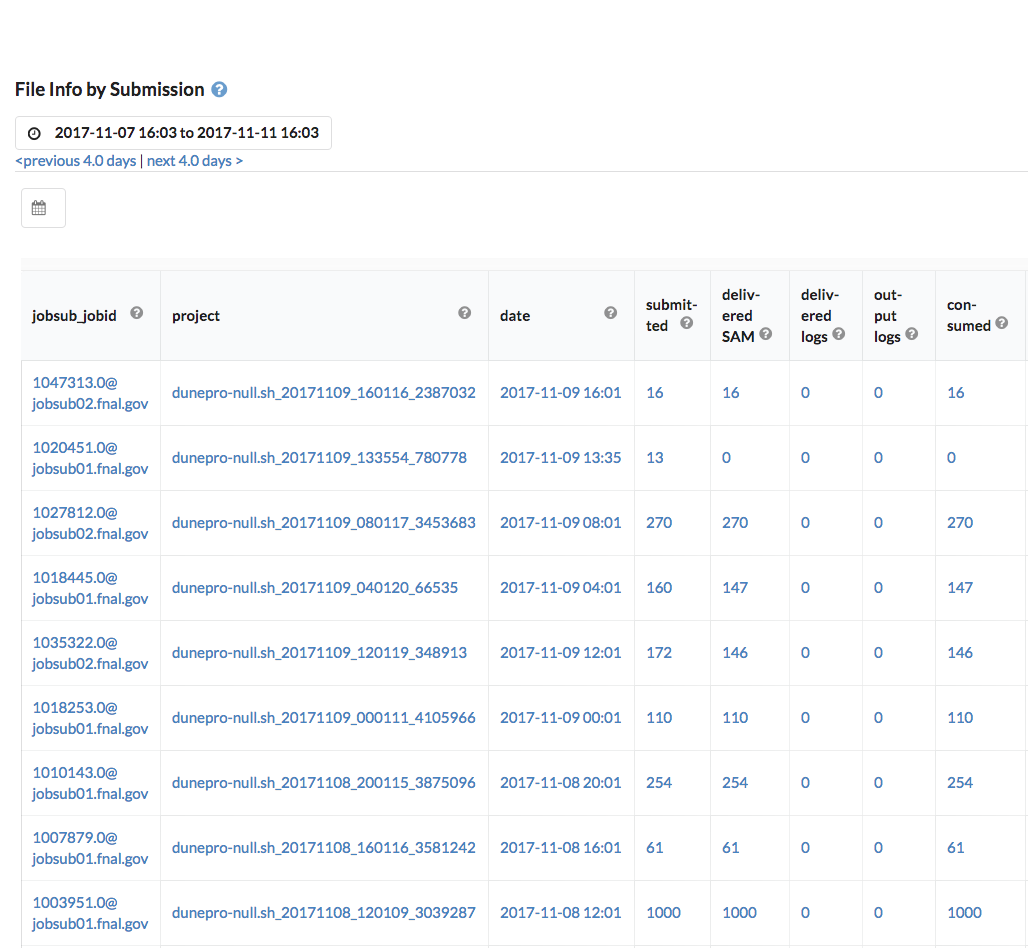
\includegraphics[width=0.8\textwidth]{./ReportImages/DC1_Phase1.png}
  \caption{POMS Monitoring of Phase 1 of Keepup Processing}
  \label{fig:keepupprocessingphase1}
\end{figure}

\item Phase 2 : Copy in then  Copy out, using LarSoft executable where the algorithm code is just a 7 min sleep. \\
This phase was affected by a significant slowness of dCache due to another process that was deleting a non-empty directory through gridftp at a rate over 500-700 operations/minute. \\
The Phase 2 processing started running smoothly since the midnight of November 10th.
Like the previous phase, the processing is monitored through the POMS webpages (Fig.\ref{fig:keepupprocessingphase2}) to identify problems and bottlenecks.
\pagebreak

\begin{figure}[tbh]
  \centering
  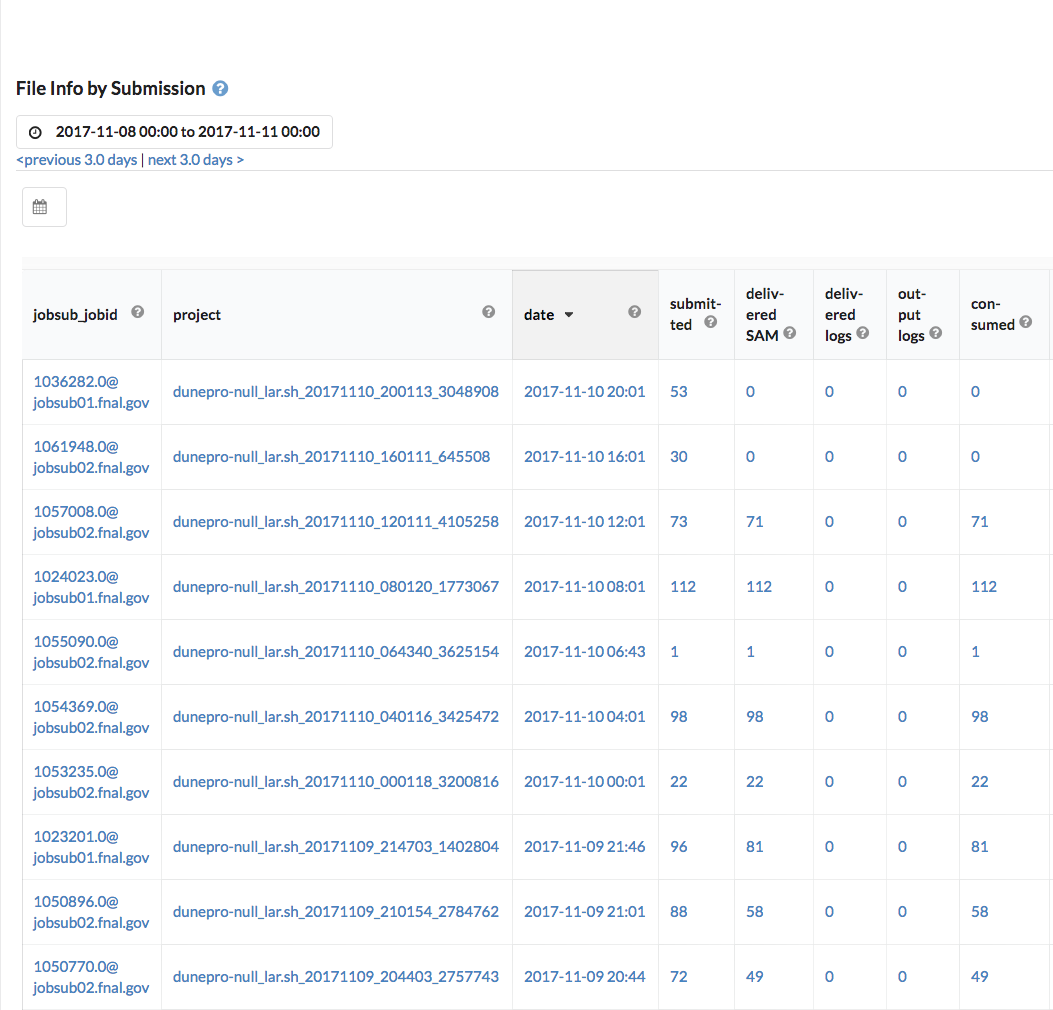
\includegraphics[width=0.8\textwidth]{./ReportImages/DC1_Phase2_2.png}
  \caption{POMS Monitoring of Phase 2 of Keepup Processing}
  \label{fig:keepupprocessingphase2}
\end{figure}

\item Phase 3: Processing of physics payloads.\\
Quite $38\%$ of 584 jobs  ($15\%$ of the data from CERN) submitted during this phase went hold  because of  time ($11\%$) and memory limit ($27\%$) issues.
The memory and the time requested were 4000 MB and 12 hrs respectively.
The keepup was put  on hold for further investigation.
POMS monitoring webpage is shown in Fig.\ref{fig:keepupprocessingphase3}.

\begin{figure}[tbh]
  \centering
  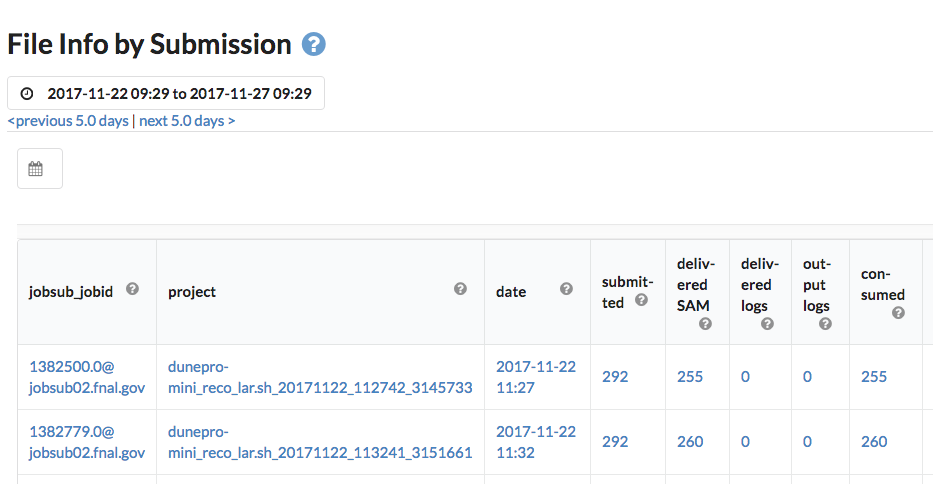
\includegraphics[width=0.8\textwidth]{./ReportImages/DC1_Phase3.png}
  \caption{POMS Monitoring of Phase 3of Keepup Processing}
  \label{fig:keepupprocessingphase3}
\end{figure}

The resource usage from the profiling CI validation of the Phase 3 dataset with an increased request of time and memory (24 hrs and 8000 MB) is shown in Fig.\ref{fig:ciphase3}.

\begin{figure}[tbh]
  \centering
  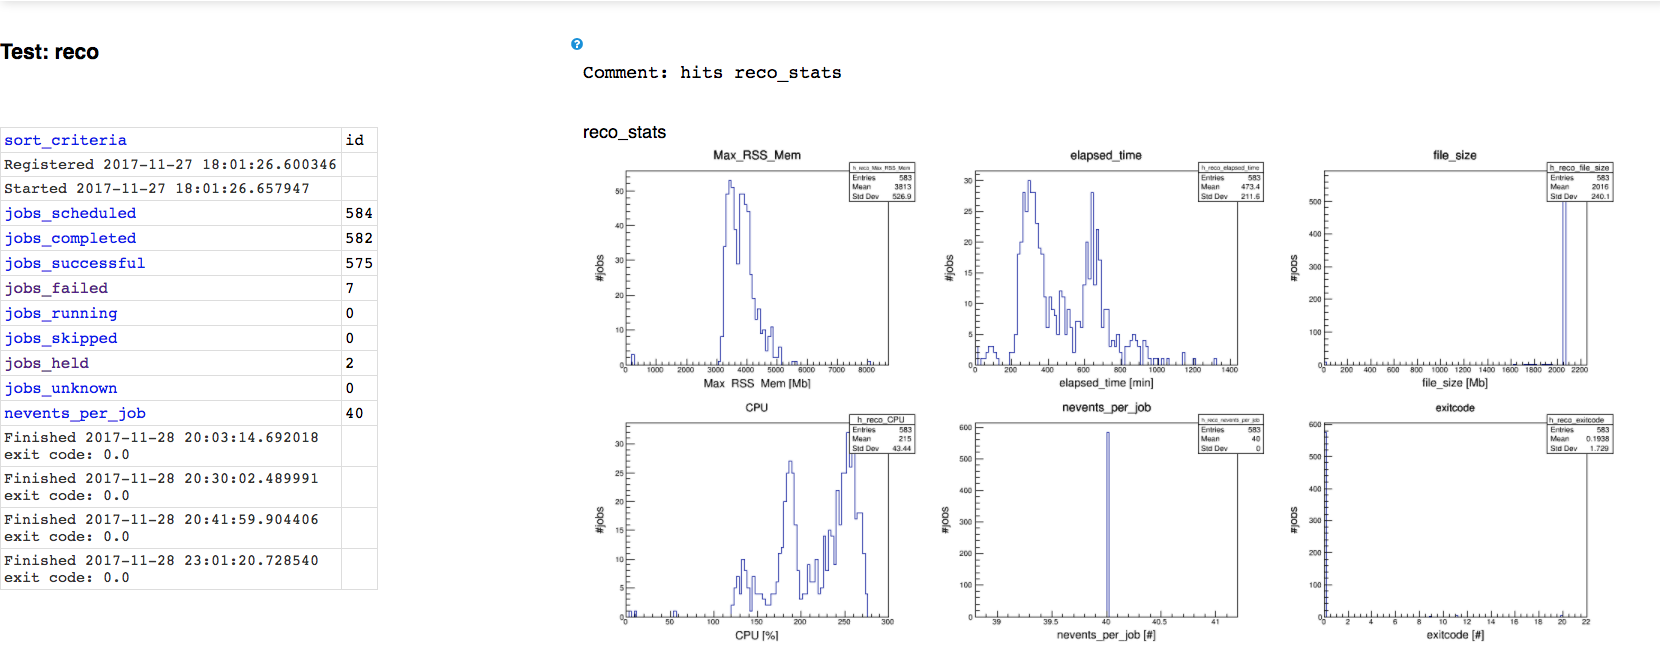
\includegraphics[width=0.8\textwidth]{./ReportImages/DC1_Phase3_CI.png}
  \caption{Continuous Integration webpage}
  \label{fig:ciphase3}
\end{figure}

\end{itemize}

In summary: \\
1 job exceeded the required memory (8000MB),
1 job exceeded the expected lifetime (24h),
4 jobs crashed with a segmentation violation,
3 jobs failed to access the input file,
582 jobs used up to  5800MB of memory and needed  22.3 hours  to complete 583 jobs, more details are in the CI webpage plots.\\
The average processing time per file was 8 hours (~12min/event).  Each file contained ~40 events, corresponding to about 1.6 seconds of ProtoDUNE-SP running (at the nominal 25 Hz rate).


\pagebreak

\subsection {Sam Projects and File Copy Status}

The pool of files available for delivery, and the collection of processes pulling files from the pool are described by  SAM projects.
Last SAM Project of Phase 2 (Submission @ 4am CST)

\href{http://samweb.fnal.gov:8480/station_monitor/dune/stations/dune/projects/dunepro-null_lar.sh_20171110_040116_3425472}{Sam Catalog}



\begin{figure}[tbh]
  \centering
  \includegraphics[width=0.5\textwidth]{./ReportImages/SamProjectsKeepupoutput.jpg}
  \caption{Monitoring of File Movement During Keep Up Processing}
  \label{fig:FTSKeepUPProcessing}
\end{figure}



\begin{figure}[tbh]
  \centering
  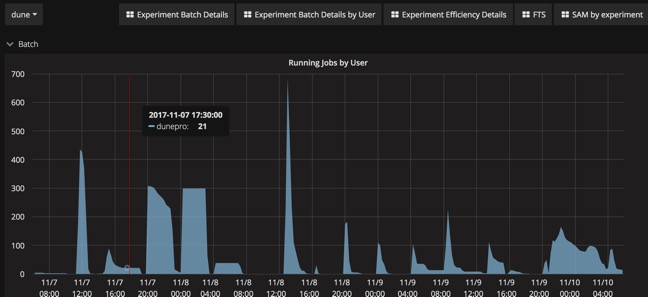
\includegraphics[width=0.5\textwidth]{./ReportImages/FIFEMonkeepup.jpg}
  \caption{Monitoring of Batch Jobs associated with Keep Up Processing}
  \label{fig:FIFEmon}
\end{figure}



\section {Beam Instrumentation}

Two parts of the beam instrumentation infrastructure were tested. The first is for sustained transfer data from an existing DIP (LHC) service at CERN to the IFBEAM database instance at Fermilab. The second is to ingest fake protoDUNE beam instrumentation data to the IFBEAM database and then read it back out into a data processing job using the LArSoft framework. 


\subsection {Ingest from DIP Service}

A Collector was developed and deployed on protodune-bidb-dev virtual machine. The collector was reading 32 LHC Beam Position monitor devices from DIP server. There were constantly 2 redundant collectors running, so they
duplicated the information. They wrote data in a format ingestible into IFBeam DB. These files were sent to FNAL using rsync with Kerberos client authentication. At FNAL, they were ingested into the production IFBeam
database. Total redundant data traffic was about 2.4MB per minute uncompressed. Our estimate for production data rate for ProtoDUNE is 48 KB/sec or about 2.8 MB/minute for single collector, or about 6 MB/sec for 2 redundant
collectors. We believe the network link will not be a problem here when we scale to the production rate. 

All CERN data is currently stored as short-term data only.   Meaning the database will only retain it for a month.   We are leaving it like this until we start taking production, long-term, data.   As we near production, it will be very important that we know when to switch.  Even though this data is ?noise?, we would like to keep it running for testing purposes.
\subsection {Fake data test}
 This data is being stored as long-term stored under a different "event" to distinguish it from production.

\section {Collaboration Tools}
\begin {itemize}
\item SLACK Channel
We successfully used a data challenge slack channel to communicate ongoing work and issues encountered. 
\item  wiki monitoring links
We used a
\href {wiki.dunescience.org} page to link to monitoring and documentation information relevant to operations of the data challenge. 
\item physical and virtual rooms 
we were more or less successful in having  a regular meeting using zoom as part of the challenge. Since only Maxim travelled to CERN for this data challenge the use of a physical meeting room was less successful


\section {Conclusion from Data Challenge 1}

Much progress was made during the week that  will stand in good stead for ramping up the whole system to the full data rate and sustainability needed for commissioning and beam running in 2018. 

\section {Input to the Joint Data Challenge Planning}
Following the work on DC1 the  agreement is to have a Joint Data Challenge in March 2018 as a collaboration between ProtoDUNE Single Phase (NP04) and ProtoDUNE Dual Phase (NP02). In January we plan a DC1.5 to test the throughput from the NP04 DAQ Online storage buffer to EOS and to do a preliminary test of the EOS access patterns. 

The data challenge will include

\begin{itemize}

\item  A  test of the full data flow, archiving and processing rate + some overhead to allow for contingency in cosmic ray and beam data volumes as well as event processing times. 

\item Event data files read out from the detector; this will necessarily be a subset of the full detector as only some detector readout elements will be present to this schedule.

\item Test of the managament and sharing features of the system at CERN, including the Tier-0 compute farm, the EHN1 networking etc. 

\item Operations processes, monitoring, notification and response. This will include having all offline services running as "DUNE services". 


\item  Identification and,  if possible,  testing of "fall back" and redundancy features  

\end{itemize}



\end{itemize}





\clearpage



\end{document}

%%% Local Variables:
%%% mode: latex
%%% TeX-master: t
%%% End:
\grid
